\documentclass[12pt, addpoints]{exam/exam}

\usepackage{hyperref}
%\usepackage{mdframed}
\usepackage{graphicx, caption}	
%\usepackage{array, multicol, tabu}
\usepackage{amsmath, amsthm, amssymb}
\usepackage{comment}
\usepackage{enumitem}
\usepackage{url}
\usepackage{textcomp}
\usepackage{wrapfig}
\newcommand{\1}{^{-1}}
\newcommand{\vect}[1]{\mathbf{#1}}
\newcommand{\R}{\mathbb R}
\newcommand{\vstr}{\vspace{\stretch{1}}}
\everymath{\displaystyle}
\setlength{\parindent}{0pt}

\theoremstyle{plain}
\newtheorem{thm}{Theorem}
\newtheorem*{thm*}{Theorem}

%\printanswers
\pointformat{\bf(\thepoints)}
\pointpoints{pt}{pts}
\bonuspointformat{\bf(\thepoints)}
\bonuspointpoints{pt}{pts}

\coverfirstpageheader{\bf MATH 236 (Calculus II) \\
		Fall 2017 \\
		}
		{}
		{{Name:} \underline{\hspace{40ex}} \\
		\vspace{0.5pc}
		Tues 31 Oct 2017}
\coverextraheadheight[2pc]{0in}
\coverfirstpagefooter{}{}{\Large Good luck!}
\coverrunningheader{}
	{Exam 2: Sequences and series}
	{}
\coverrunningheadrule	
\coverrunningfootrule
\coverrunningfooter{Calc II Fall 2017}{}{p. \thepage\ (of \numpages)}

\firstpageheader{}
	{Exam 2: Sequences and series}
	{}
\firstpageheadrule
\firstpagefootrule
\firstpagefooter{Calc II Fall 2017}{}{p. \thepage\ (of \numpages)}

\runningheadrule
\runningheader{}
	{Exam 2: Sequences and series}
	{}
\runningfootrule
\runningfooter{Calc II Fall 2017}{}{p. \thepage\ (of \numpages)}

\title{\vspace{-8pc}
\vfill{\Huge
	\bf Exam 2: Sequences and series \\ 
	(\S5.6, 7.1-7.7)} 
	}
%\author{}
\date{}

% % % % % % % % % % % % % % % % % % % %
\begin{document}

\begin{coverpages}
\maketitle
\thispagestyle{headandfoot}
\vspace{-4pc}
{\bf Exam Instructions:} You have 75 minutes to complete this exam.  Justification is required for all problems.  Notation matters!  You will also be penalized for missing units and rounding errors.  
No electronic devices (phones, iDevices, computers, etc) except for a \textbf{basic scientific calculator}.  On story problems, round to two decimal places. 

\vspace{1pc}
If you finish early then you may leave, UNLESS there are less than 5 minutes of class left.  To prevent disruption, if you finish with less than 5 minutes of class remaining then please stay seated and quiet.

\begin{flushright}
%In addition, please provide the following data:

\vspace{0.3in}
%Drill Instructor: \underline{\hspace{40ex}}

\vspace{0.3in}
%Drill Time: \underline{\hspace{40ex}}
\end{flushright}

\vfill
\textbf{Your signature below indicates that you have read this page and agree to follow the Academic Honesty Policies of James Madison University.}  

\vspace{0.3in}
Signature: {\bf (1 pt)} \underline{\hspace{73ex}}

% % % % % % % % % %
\newpage
\vspace*{\fill}
\gradetable
%\textbf{Formulas you may need:}
%\vspace{-2pc}
%\begin{center}
%\vspace*{\fill}
%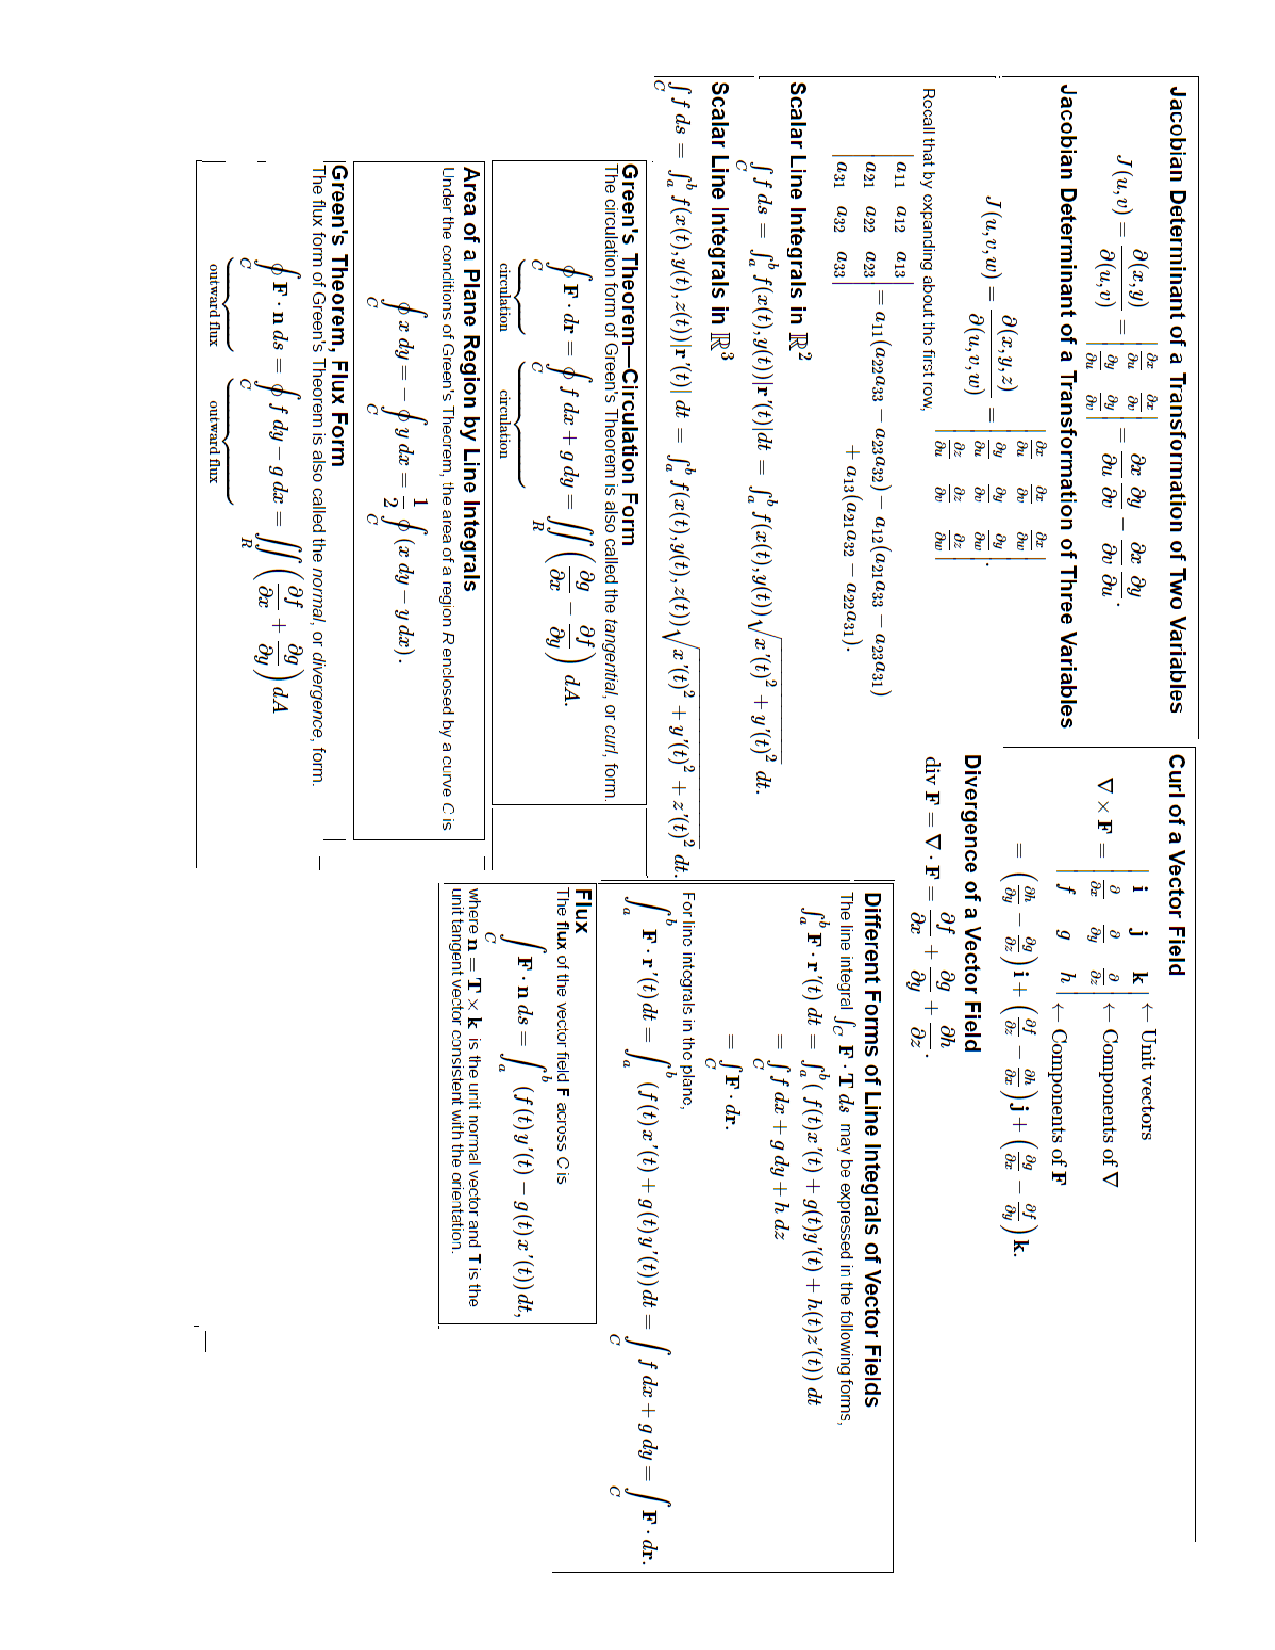
\includegraphics[scale=0.84]{Exam3FormulaSheet.pdf}
%\vspace*{\fill}
%\end{center}
\end{coverpages}

% % % % % % % % % % % % % % % % % % % %
\begin{questions}
\thispagestyle{headandfoot}

% % % % %
\question[12] %{\bf 7.1 \#20}
Find a plausible formula for the general term of the sequence 
\[
\left\{1,\frac{1}{2},\frac{1}{6},\frac{1}{24},\frac{1}{120},\dots\right\}.
\]
Assume the indexing starts at $k=-1$.
\vfill

\newpage
% % % % % 
\question%[] %{\bf CR \#6}
Consider the sequence $\sigma=\left\{\sin\left(\frac{\pi}{2k}\right)\right\}_{k=1}^{\infty}$.
	\begin{parts}
	\part[2] Write the first five terms of $\sigma$.
	\vspace{5pc}

	\part[3] Determine whether $\sigma$ is monotone.  If so, is it strict?  Is it eventual?
	%\vspace{8pc}
	\vfill

	\part[4] Determine the least upper bound and greatest lower bound for $\sigma$.
	%\vspace{8pc}
	\vfill

	\part[4] Explain why $\sigma$ must converge and then find what it converges to.
	\vfill

	\end{parts}

\newpage
% % % % %
\question %{\bf CR \#10} 
Consider the series $S=\sum_{k=0}^{\infty}\left(\frac{2^k}{(k+3)!}-\frac{2^{k+1}}{(k+4)!}\right)$.
	\begin{parts}
	\part[3] Write the first five partial sums $S_0$, $S_1$, $S_2$, $S_3$, $S_4$.
	\vspace{18pc}
	
	\part[4] Write a closed formula for the general partial sum $S_n$.
	\vfill
	
	\part[4] Evaluate $\lim_{n\to\infty}S_n$.
	\vfill
	
	\part[3] What is the sum of the series $S$?
	\vspace{4pc}
	\end{parts}

\newpage
% % % % %
\question[15] %{\bf CR \#24}	
Determine whether the series $\sum_{k=0}^{\infty}\frac{5^k+k}{k!+3}$ converges or diverges.  You may need to employ a battery of tests; explain the criteria you are using and why your conclusion is valid.

\newpage
% % % % %
\question[15] %{\bf CR \#32}
Determine whether the series $\sum_{k=1}^{\infty}\frac{(-1)^k}{\sqrt{k(1+k)}}$ converges absolutely, converges conditionally, or diverges.  Explain the criteria you are using and why your conclusion is valid.

\newpage
% % % % %
\question[15] %{\S5.6 \#52}
Evaluate $\int_0^1\frac{dx}{x(x-1)}$.  \textit{Note: This is an improper integral.  You will be penalized for not using limits in your answer.}

\newpage
% % % % %
\question[15] %{\S7.3 \#80}
Prof Wheeler drops a ping pong ball from a height of 1 meter.  Each time it bounces, it only rebounds to $p$\% (where $0<p<100$) of its previous height.  Draw a diagram illustrating the problem.  Then use a series to determine the total up and down distance the ball travels.

\end{questions}

\end{document}